\documentclass[aps,prb,onecolumn,nofootinbib,superscriptaddress]{revtex4-2}
\usepackage{amsmath,amssymb,amsthm,mathtools,bm}
\usepackage{booktabs,graphicx}
\usepackage[colorlinks=true,linkcolor=blue,citecolor=blue,urlcolor=blue]{hyperref}
\usepackage{microtype}
\begin{document}
\title{Late-time slope diagnostics from saved slab-only purification histories}
\date{8 October 2026}
\begin{abstract}
We analyze existing 100-trajectory slab-only ensembles at seven circumferences through four times the circumference. Paired endpoint differences and late-window linear fits give finite-time size exponents close to one. The analysis removes a constant raw-gap offset under an affine-growth assumption; it does not establish an infinite-time Lyapunov gap. No new dynamics are simulated, and no manuscript gap claims are changed.
\end{abstract}
\maketitle
\setcounter{tocdepth}{2}
\tableofcontents
\section{Estimators and uncertainty}
For each record, the saved raw modular gap is the minimum absolute modular energy, with pinned occupations excluded using the original extraction tolerance $10^{-9}$:
\begin{equation}
g_{\rm mod}(t)=\min_j\left|\log\frac{1-\nu_j(t)}{\nu_j(t)}\right|=2t\Delta(t).
\end{equation}
The independent sampling unit is a trajectory. For each of the 100 trajectories at each circumference, compute
\begin{equation}
\Delta_{\rm late}=\frac{g_{\rm mod}(4N_y)-g_{\rm mod}(3N_y)}{2N_y}.
\end{equation}
The primary estimate is its ensemble mean, with ordinary trajectory SEM. This retains temporal correlations automatically. A comparison estimator is half the unweighted least-squares slope of $g_{\rm mod}$ on all saved cycles in $[3N_y,4N_y]$, with a free intercept, computed separately per trajectory and then averaged with its SEM. Endpoint differences and multi-time fits are different estimators. No bootstrap is used.
All data use $N_x=20$, $\alpha_1=1$, $\alpha_2=30$, and the saved slab-only protocol with a maximally mixed slab and Born-prepared exterior. Full-measurement histories are not pooled. Source receipts, trajectory IDs, and the relation $g_{\rm mod}=2t\Delta$ were verified in the existing extraction; this analysis verifies the sample-history checksum and complete paired records.
\section{Size comparison}
\begin{table}[h]
\caption{Ensemble means with one trajectory SEM. All entries are finite-window rates.}
\begin{ruledtabular}\begin{tabular}{rrrr}
$N_y$ & $\overline\Delta(2N_y)$ & Endpoint slope & Fitted slope\\
20 & $0.04136\pm0.00248$ & $0.06688\pm0.00629$ & $0.06534\pm0.00653$ \\
24 & $0.03736\pm0.00185$ & $0.05912\pm0.00468$ & $0.05767\pm0.00460$ \\
30 & $0.02803\pm0.00146$ & $0.04395\pm0.00364$ & $0.04365\pm0.00383$ \\
36 & $0.02234\pm0.00141$ & $0.03459\pm0.00310$ & $0.03354\pm0.00322$ \\
44 & $0.01790\pm0.00091$ & $0.02872\pm0.00249$ & $0.02770\pm0.00270$ \\
56 & $0.01467\pm0.00080$ & $0.02186\pm0.00194$ & $0.02200\pm0.00214$ \\
60 & $0.01317\pm0.00072$ & $0.02255\pm0.00194$ & $0.02158\pm0.00206$ \\
\end{tabular}\end{ruledtabular}\end{table}
The fits use $\log\Delta=\log A-z\log N_y$, with propagated log-space SEMs $\sigma_{\log\Delta}=\mathrm{SEM}/\Delta$. Exponent errors are the formal weighted-regression covariance errors from these supplied uncertainties, without rescaling by residual scatter.
\begin{align}
z_{2N_y} &= 1.0788\pm 0.0540,\qquad \chi^2/\mathrm{dof}=0.489,\nonumber\\
z_{\mathrm{endpoint}} &= 1.0682\pm 0.0859,\qquad \chi^2/\mathrm{dof}=0.332,\nonumber\\
z_{\mathrm{fit}} &= 1.0751\pm 0.0921,\qquad \chi^2/\mathrm{dof}=0.238.
\end{align}
\begin{figure}[h]
\centering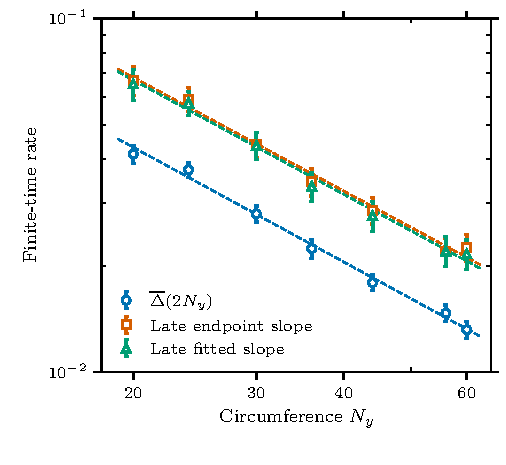
\includegraphics[width=3.375in]{late_gap_comparison.pdf}
\caption{Saved slab-only finite-time rates versus circumference. Bars are paired trajectory SEMs; dashed curves are separate SEM-weighted power-law fits. All 100 trajectories are retained at each size.}
\end{figure}
\section{Interpretation and limits}
Both late-window estimators support an approximately inverse-circumference trend over the seven saved sizes, rather than an evident size-independent plateau. Under $g_{\rm mod}(t)\simeq at+b$, a slope removes the constant offset $b$ and yields $a/2$, whereas $\Delta(t)$ contains $b/(2t)$. This cancellation is conditional on approximately affine growth over the selected window. The two slope estimates differ by less than 1.4 paired SEM at every size.
The late estimates exceed $\overline\Delta(2N_y)$, consistent with the previously observed drift. Their agreement in size exponent strengthens the finite-time evidence: the observed trend is not removed by subtracting a constant raw-gap offset. However, the minimizing mode can change with cycle, and the observation windows themselves grow with $N_y$. These are not established asymptotic exponents or infinite-time gaps. No new results have been inserted into Figures 4 or A2, or used to change the section title or gap claims.
\end{document}
